% Chapter 10: Comprehensive Review - Complete Time Series Analysis
% Applying all methods to real data: Bitcoin, Sunspots, Unemployment
% Bachelor program, Bucharest University of Economic Studies

\documentclass[9pt, aspectratio=169, t]{beamer}

% Ensure content fits on slides
\setbeamersize{text margin left=8mm, text margin right=8mm}

%=============================================================================
% THEME AND STYLE CONFIGURATION
%=============================================================================
\usetheme{Madrid}
\usecolortheme{seahorse}

% IDA-Inspired Color Palette
\definecolor{MainBlue}{RGB}{26, 58, 110}
\definecolor{AccentBlue}{RGB}{42, 82, 140}
\definecolor{IDAred}{RGB}{220, 53, 69}
\definecolor{DarkGray}{RGB}{51, 51, 51}
\definecolor{MediumGray}{RGB}{128, 128, 128}
\definecolor{LightGray}{RGB}{248, 248, 248}
\definecolor{VeryLightGray}{RGB}{235, 235, 235}
\definecolor{Crimson}{RGB}{220, 53, 69}
\definecolor{Forest}{RGB}{46, 125, 50}
\definecolor{Amber}{RGB}{181, 133, 63}
\definecolor{Orange}{RGB}{230, 126, 34}
\definecolor{BitcoinOrange}{RGB}{247, 147, 26}

\setbeamercolor{palette primary}{bg=MainBlue, fg=white}
\setbeamercolor{palette secondary}{bg=MainBlue!85, fg=white}
\setbeamercolor{palette tertiary}{bg=MainBlue!70, fg=white}
\setbeamercolor{structure}{fg=MainBlue}
\setbeamercolor{title}{fg=MainBlue}
\setbeamercolor{frametitle}{fg=MainBlue, bg=white}
\setbeamercolor{block title}{bg=MainBlue, fg=white}
\setbeamercolor{block body}{bg=VeryLightGray, fg=DarkGray}
\setbeamercolor{block title alerted}{bg=Crimson, fg=white}
\setbeamercolor{block body alerted}{bg=Crimson!8, fg=DarkGray}
\setbeamercolor{block title example}{bg=Forest, fg=white}
\setbeamercolor{block body example}{bg=Forest!8, fg=DarkGray}
\setbeamercolor{item}{fg=MainBlue}

\setbeamertemplate{navigation symbols}{}

\setbeamertemplate{footline}{
    \leavevmode%
    \hbox{%
        \begin{beamercolorbox}[wd=.333333\paperwidth,ht=2.5ex,dp=1ex,center]{author in head/foot}%
            \usebeamerfont{author in head/foot}\insertshortauthor
        \end{beamercolorbox}%
        \begin{beamercolorbox}[wd=.333333\paperwidth,ht=2.5ex,dp=1ex,center]{title in head/foot}%
            \usebeamerfont{title in head/foot}\insertshorttitle
        \end{beamercolorbox}%
        \begin{beamercolorbox}[wd=.333333\paperwidth,ht=2.5ex,dp=1ex,right]{date in head/foot}%
            \usebeamerfont{date in head/foot}\insertshortdate{}\hspace*{2em}
            \insertframenumber{} / \inserttotalframenumber\hspace*{2ex}
        \end{beamercolorbox}}%
    \vskip0pt%
}

%=============================================================================
% PACKAGES
%=============================================================================
\usepackage[utf8]{inputenc}
\usepackage[T1]{fontenc}
\usepackage{amsmath, amssymb, amsthm}
\usepackage{mathtools}
\usepackage{bm}
\usepackage{tikz}
\usetikzlibrary{arrows.meta, positioning, shapes, calc}
\usepackage{booktabs}
\usepackage{multirow}
\usepackage{array}
\usepackage{graphicx}
\usepackage{hyperref}
\hypersetup{colorlinks=false, pdfborder={0 0 0}}
\graphicspath{{../logos/}{../charts/}}

%=============================================================================
% THEOREM ENVIRONMENTS
%=============================================================================
\theoremstyle{definition}
\setbeamertemplate{theorems}[numbered]
\newtheorem{defn}{Definition}
\newtheorem{thm}{Theorem}
\newtheorem{prop}{Proposition}

%=============================================================================
% CUSTOM COMMANDS
%=============================================================================
\newcommand{\E}{\mathbb{E}}
\newcommand{\Var}{\text{Var}}
\newcommand{\Cov}{\text{Cov}}
\newcommand{\Corr}{\text{Corr}}
\newcommand{\R}{\mathbb{R}}

%=============================================================================
% TITLE INFORMATION
%=============================================================================
\title[Chapter 10: Comprehensive Review]{Chapter 10: Comprehensive Review}
\subtitle{Bachelor Program, Faculty of Cybernetics, Statistics and Economic Informatics, Bucharest University of Economic Studies}
\author[Prof. Daniel Traian Pele, PhD]{Prof. Daniel Traian Pele, PhD\\[0.2cm]\footnotesize\texttt{danpele@ase.ro}}
\institute{Bucharest University of Economic Studies}
\date{Academic Year 2025--2026}

\begin{document}

%=============================================================================
% TITLE SLIDE
%=============================================================================
\begin{frame}[plain]
    \begin{tikzpicture}[remember picture, overlay]
        \fill[IDAred] (current page.north west) rectangle ([yshift=-0.15cm]current page.north east);
        \node[anchor=north west] at ([xshift=0.5cm, yshift=-0.3cm]current page.north west) {
            \href{https://www.ase.ro}{\includegraphics[height=1.1cm]{ase_logo.png}}
        };
        \node[anchor=north] at ([yshift=-0.3cm]current page.north) {
            \href{https://ai4efin.ase.ro}{\includegraphics[height=1.1cm]{ai4efin_logo.png}}
        };
        \node[anchor=north east] at ([xshift=-0.5cm, yshift=-0.3cm]current page.north east) {
            \href{https://www.digital-finance-msca.com}{\includegraphics[height=1.1cm]{msca_logo.png}}
        };
    \end{tikzpicture}
    \vfill
    \begin{center}
        {\Large\textcolor{MediumGray}{Time Series Analysis and Forecasting}}\\[0.3cm]
        {\Huge\textbf{\textcolor{MainBlue}{Chapter 10: Comprehensive Review}}}\\[0.5cm]
        {\Large\textcolor{IDAred}{Complete Analysis with Real Data}}
    \end{center}
    \vfill

    \begin{tikzpicture}[remember picture, overlay]
        \fill[IDAred] (current page.south west) rectangle ([yshift=0.15cm]current page.south east);
        \node[anchor=south west] at ([xshift=0.5cm, yshift=0.8cm]current page.south west) {
            \href{https://theida.net}{\includegraphics[height=0.9cm]{ida_logo.png}}
        };
        \node[anchor=south] at ([xshift=-3cm, yshift=0.8cm]current page.south) {
            \href{https://blockchain-research-center.com}{\includegraphics[height=0.9cm]{brc_logo.png}}
        };
        \node[anchor=south] at ([yshift=0.8cm]current page.south) {
            \href{https://quantinar.com}{\includegraphics[height=0.9cm]{qr_logo.png}}
        };
        \node[anchor=south] at ([xshift=3cm, yshift=0.8cm]current page.south) {
            \href{https://quantlet.com}{\includegraphics[height=0.9cm]{ql_logo.png}}
        };
        \node[anchor=south east] at ([xshift=-0.5cm, yshift=0.8cm]current page.south east) {
            \href{https://ipe.ro/new}{\includegraphics[height=0.9cm]{acad_logo.png}}
        };
    \end{tikzpicture}
\end{frame}

%=============================================================================
% TABLE OF CONTENTS
%=============================================================================
\begin{frame}{Outline}
    \tableofcontents
\end{frame}

%=============================================================================
% SECTION 1: INTRODUCTION
%=============================================================================
\section{The Complete Analysis Workflow}

\begin{frame}{Course Overview: Methods Covered}
    \begin{columns}[T]
        \begin{column}{0.48\textwidth}
            \textbf{Classical Methods}
            \begin{itemize}
                \item \textcolor{MainBlue}{Ch 1:} Time Series Fundamentals
                \item \textcolor{MainBlue}{Ch 2:} ARMA Models
                \item \textcolor{MainBlue}{Ch 3:} ARIMA Models
                \item \textcolor{MainBlue}{Ch 4:} SARIMA Models
                \item \textcolor{MainBlue}{Ch 5:} GARCH Models
            \end{itemize}
        \end{column}
        \begin{column}{0.48\textwidth}
            \textbf{Advanced Methods}
            \begin{itemize}
                \item \textcolor{Forest}{Ch 6:} VAR \& Granger Causality
                \item \textcolor{Forest}{Ch 7:} Cointegration \& VECM
                \item \textcolor{Forest}{Ch 8:} Modern Extensions
                \item \textcolor{Forest}{Ch 9:} Prophet \& TBATS
            \end{itemize}
            \vspace{0.5em}
            \textbf{Today: Apply ALL to Real Data!}
        \end{column}
    \end{columns}
\end{frame}

\begin{frame}{The Complete Analysis Workflow}
    \begin{center}
        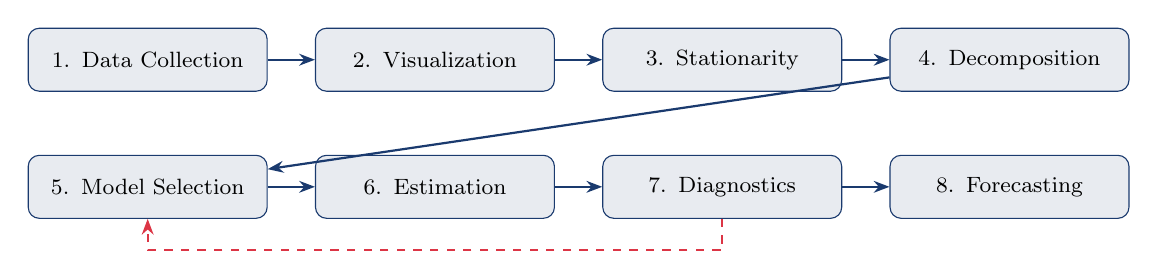
\begin{tikzpicture}[
            node distance=0.6cm,
            box/.style={rectangle, rounded corners, draw=MainBlue, fill=MainBlue!10,
                        text width=2.8cm, minimum height=0.8cm, align=center, font=\footnotesize},
            arrow/.style={-{Stealth[length=2mm]}, thick, MainBlue}
        ]
            % Row 1
            \node[box] (data) {1. Data Collection};
            \node[box, right=of data] (viz) {2. Visualization};
            \node[box, right=of viz] (stat) {3. Stationarity};
            \node[box, right=of stat] (decomp) {4. Decomposition};

            % Row 2
            \node[box, below=0.8cm of data] (model) {5. Model Selection};
            \node[box, right=of model] (est) {6. Estimation};
            \node[box, right=of est] (diag) {7. Diagnostics};
            \node[box, right=of diag] (forecast) {8. Forecasting};

            % Arrows
            \draw[arrow] (data) -- (viz);
            \draw[arrow] (viz) -- (stat);
            \draw[arrow] (stat) -- (decomp);
            \draw[arrow] (decomp) -- (model);
            \draw[arrow] (model) -- (est);
            \draw[arrow] (est) -- (diag);
            \draw[arrow] (diag) -- (forecast);

            % Feedback loop
            \draw[arrow, dashed, IDAred] (diag.south) -- ++(0,-0.4) -| (model.south);
        \end{tikzpicture}
    \end{center}

    \vspace{0.3cm}
    \begin{alertblock}{Key Principle}
        Model diagnostics may require returning to model selection (iterative process)
    \end{alertblock}
\end{frame}

\begin{frame}{Real Datasets for This Chapter}
    \begin{columns}[T]
        \begin{column}{0.24\textwidth}
            \begin{block}{\textcolor{BitcoinOrange}{Bitcoin}}
                \begin{itemize}
                    \item Daily 2019-2024
                    \item Volatility clustering
                    \item ARIMA + GARCH
                \end{itemize}
            \end{block}
        \end{column}
        \begin{column}{0.24\textwidth}
            \begin{block}{\textcolor{Orange}{Sunspots}}
                \begin{itemize}
                    \item Yearly 1900-2023
                    \item 11-year cycle
                    \item Fourier terms
                \end{itemize}
            \end{block}
        \end{column}
        \begin{column}{0.24\textwidth}
            \begin{block}{\textcolor{MainBlue}{Unemployment}}
                \begin{itemize}
                    \item Monthly 2010-2023
                    \item COVID-19 shock
                    \item Prophet
                \end{itemize}
            \end{block}
        \end{column}
        \begin{column}{0.24\textwidth}
            \begin{block}{\textcolor{Forest}{Economic VAR}}
                \begin{itemize}
                    \item Quarterly 2000-2023
                    \item GDP, Inflation, etc.
                    \item Multivariate VAR
                \end{itemize}
            \end{block}
        \end{column}
    \end{columns}
\end{frame}

%=============================================================================
% TRAIN/VALIDATION/TEST METHODOLOGY
%=============================================================================
\begin{frame}{Key Methodology: Train / Validation / Test Split}
    \begin{center}
        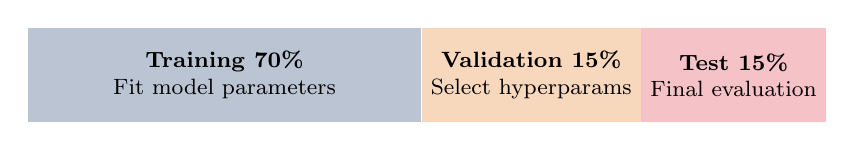
\begin{tikzpicture}[
            box/.style={rectangle, minimum height=1.2cm, align=center, font=\footnotesize},
        ]
            \node[box, fill=MainBlue!30, minimum width=5cm] (train) at (0,0) {\textbf{Training 70\%}\\Fit model parameters};
            \node[box, fill=Orange!30, minimum width=2.2cm, right=-0.01cm of train] (val) {\textbf{Validation 15\%}\\Select hyperparams};
            \node[box, fill=IDAred!30, minimum width=2.2cm, right=-0.01cm of val] (test) {\textbf{Test 15\%}\\Final evaluation};
        \end{tikzpicture}
    \end{center}

    \vspace{0.3em}
    \begin{columns}[T]
        \begin{column}{0.48\textwidth}
            \textbf{Why This Matters:}
            \begin{itemize}
                \item \textcolor{MainBlue}{Training}: Estimate model parameters
                \item \textcolor{Orange}{Validation}: Compare models, tune hyperparameters
                \item \textcolor{IDAred}{Test}: Unbiased final performance (held out!)
            \end{itemize}
        \end{column}
        \begin{column}{0.48\textwidth}
            \begin{alertblock}{Critical Rule}
                \textbf{NEVER} look at test data during model selection!

                \vspace{0.2em}
                For time series: \textbf{NEVER} shuffle data --- preserve temporal order.
            \end{alertblock}
        \end{column}
    \end{columns}
\end{frame}

%=============================================================================
% SECTION 2: CASE STUDY 1 - BITCOIN
%=============================================================================
\section{Case Study 1: Bitcoin Volatility Forecasting}

\begin{frame}{Bitcoin: Data and Objective}
    \begin{columns}[T]
        \begin{column}{0.55\textwidth}
            \textbf{Data:} Bitcoin daily returns (2019--2024)
            \begin{itemize}
                \item Source: Yahoo Finance (BTC-USD)
                \item 1,826 observations
                \item Returns = $100 \times \ln(P_t/P_{t-1})$
            \end{itemize}

            \vspace{0.5em}
            \textbf{Objective:} Forecast \textcolor{IDAred}{volatility} (not returns!)

            \vspace{0.5em}
            \textbf{Why volatility?}
            \begin{itemize}
                \item Returns are nearly unpredictable
                \item Volatility shows strong persistence
                \item Critical for risk management (VaR)
            \end{itemize}
        \end{column}
        \begin{column}{0.43\textwidth}
            \textbf{Data Split:}
            \begin{table}[h]
                \footnotesize
                \begin{tabular}{lcc}
                    \toprule
                    Set & Days & Period \\
                    \midrule
                    Training & 1,278 & 2019--2022 \\
                    Validation & 274 & 2022--2023 \\
                    Test & 274 & 2023--2024 \\
                    \bottomrule
                \end{tabular}
            \end{table}

            \vspace{0.5em}
            \begin{exampleblock}{Key Statistics}
                Mean return: 0.12\%/day \\
                Std dev: 3.8\%/day \\
                Kurtosis: 8.2 (fat tails!)
            \end{exampleblock}
        \end{column}
    \end{columns}
\end{frame}

\begin{frame}{Bitcoin: Model Selection on Validation Set}
    \textbf{Step 1: Fit GARCH variants on Training data}

    \textbf{Step 2: Compare volatility forecasts on Validation set}

    \vspace{0.5em}
    \begin{columns}[T]
        \begin{column}{0.55\textwidth}
            \begin{table}[h]
                \footnotesize
                \begin{tabular}{lccc}
                    \toprule
                    Model & AIC & BIC & \textbf{Val MAE} \\
                    \midrule
                    GARCH(1,1) & 8542 & 8563 & 2.34 \\
                    GARCH(2,1) & 8540 & 8567 & 2.31 \\
                    \textbf{GJR-GARCH(1,1)} & \textbf{8531} & \textbf{8558} & \textbf{2.18} \\
                    EGARCH(1,1) & 8538 & 8565 & 2.25 \\
                    \bottomrule
                \end{tabular}
            \end{table}

            \vspace{0.3em}
            \textcolor{Forest}{$\Rightarrow$ Best: GJR-GARCH (captures asymmetry)}
        \end{column}
        \begin{column}{0.43\textwidth}
            \textbf{GJR-GARCH Model:}
            \[
                \sigma_t^2 = \omega + (\alpha + \gamma I_{t-1}) \varepsilon_{t-1}^2 + \beta \sigma_{t-1}^2
            \]

            \vspace{0.3em}
            Where $I_{t-1} = 1$ if $\varepsilon_{t-1} < 0$

            \vspace{0.5em}
            \begin{alertblock}{Leverage Effect}
                $\gamma > 0$: Negative returns increase volatility more than positive returns (fear vs greed)
            \end{alertblock}
        \end{column}
    \end{columns}
\end{frame}

\begin{frame}{Bitcoin: Final Test Set Evaluation}
    \textbf{Step 3: Refit GJR-GARCH on Training+Validation, evaluate on Test}

    \vspace{0.5em}
    \begin{columns}[T]
        \begin{column}{0.48\textwidth}
            \textbf{Test Set Results:}
            \begin{table}[h]
                \footnotesize
                \begin{tabular}{lc}
                    \toprule
                    Metric & Value \\
                    \midrule
                    Volatility MAE & 2.21 \\
                    Volatility RMSE & 3.45 \\
                    \bottomrule
                \end{tabular}
            \end{table}

            \vspace{0.5em}
            \textbf{GJR-GARCH Parameters:}
            \begin{itemize}
                \item $\alpha = 0.05$ (ARCH effect)
                \item $\gamma = 0.08$ (leverage effect)
                \item $\beta = 0.89$ (persistence)
                \item $\alpha + \gamma/2 + \beta = 0.98$
            \end{itemize}
        \end{column}
        \begin{column}{0.48\textwidth}
            \textbf{Interpretation:}
            \begin{itemize}
                \item High persistence ($\approx 0.98$)
                \item Leverage effect significant ($\gamma > 0$)
                \item Volatility is predictable!
            \end{itemize}

            \vspace{0.5em}
            \begin{exampleblock}{Practical Application}
                \textbf{1-day ahead VaR (99\%):}
                \[
                    \text{VaR} = -2.33 \times \hat{\sigma}_{t+1}
                \]
                If $\hat{\sigma} = 4\%$, then VaR = $-9.3\%$
            \end{exampleblock}
        \end{column}
    \end{columns}
\end{frame}

\begin{frame}{Bitcoin: Volatility Forecast Visualization}
    \begin{center}
        \textbf{Test Period: Forecast vs Realized Volatility}

        \vspace{0.5em}
        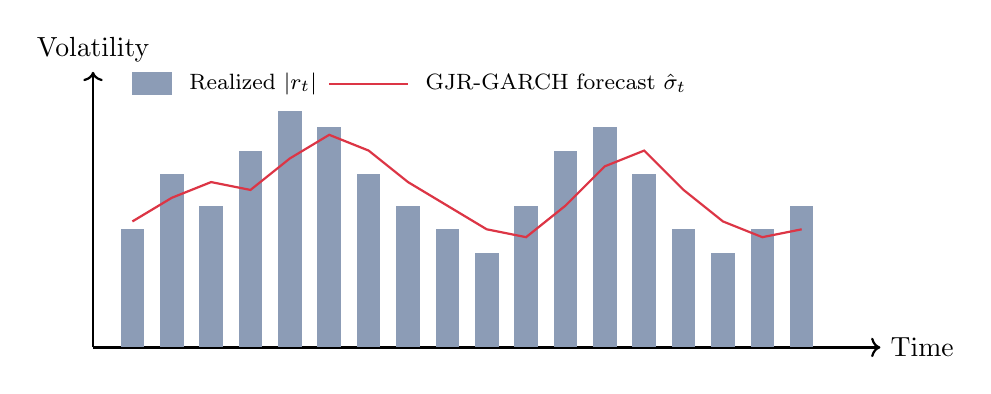
\begin{tikzpicture}
            % Simplified visualization
            \draw[thick, ->] (0,0) -- (10,0) node[right] {Time};
            \draw[thick, ->] (0,0) -- (0,3.5) node[above] {Volatility};

            % Realized volatility (bars)
            \foreach \x/\h in {0.5/1.5, 1/2.2, 1.5/1.8, 2/2.5, 2.5/3, 3/2.8, 3.5/2.2, 4/1.8, 4.5/1.5, 5/1.2, 5.5/1.8, 6/2.5, 6.5/2.8, 7/2.2, 7.5/1.5, 8/1.2, 8.5/1.5, 9/1.8} {
                \fill[MainBlue!50] (\x-0.15,0) rectangle (\x+0.15,\h);
            }

            % Forecast line
            \draw[thick, IDAred] (0.5,1.6) -- (1,1.9) -- (1.5,2.1) -- (2,2.0) -- (2.5,2.4) -- (3,2.7) -- (3.5,2.5) -- (4,2.1) -- (4.5,1.8) -- (5,1.5) -- (5.5,1.4) -- (6,1.8) -- (6.5,2.3) -- (7,2.5) -- (7.5,2.0) -- (8,1.6) -- (8.5,1.4) -- (9,1.5);

            % Legend
            \fill[MainBlue!50] (0.5,3.2) rectangle (1,3.5);
            \node[right, font=\footnotesize] at (1.1,3.35) {Realized $|r_t|$};
            \draw[thick, IDAred] (3,3.35) -- (4,3.35);
            \node[right, font=\footnotesize] at (4.1,3.35) {GJR-GARCH forecast $\hat{\sigma}_t$};
        \end{tikzpicture}
    \end{center}

    \vspace{0.3em}
    \begin{itemize}
        \item Model captures volatility clusters (high vol follows high vol)
        \item Forecast adapts to changing market conditions
        \item Test MAE = 2.21 (good for daily volatility forecasting)
    \end{itemize}
\end{frame}

\begin{frame}{Bitcoin: Summary}
    \begin{columns}[T]
        \begin{column}{0.48\textwidth}
            \textbf{Methodology:}
            \begin{enumerate}
                \item Split data: 70/15/15
                \item Compare GARCH variants on validation
                \item Select best model (GJR-GARCH)
                \item Final evaluation on test set
            \end{enumerate}

            \vspace{0.5em}
            \textbf{Key Finding:}

            Returns are unpredictable, but \textcolor{IDAred}{volatility is forecastable}!
        \end{column}
        \begin{column}{0.48\textwidth}
            \textbf{Results:}
            \begin{table}[h]
                \footnotesize
                \begin{tabular}{ll}
                    \toprule
                    Best Model & GJR-GARCH(1,1) \\
                    Validation MAE & 2.18 \\
                    Test MAE & 2.21 \\
                    Key insight & Leverage effect \\
                    \bottomrule
                \end{tabular}
            \end{table}

            \vspace{0.5em}
            \begin{exampleblock}{Practical Use}
                \begin{itemize}
                    \item Value-at-Risk calculation
                    \item Position sizing
                    \item Options pricing
                \end{itemize}
            \end{exampleblock}
        \end{column}
    \end{columns}
\end{frame}

%=============================================================================
% SECTION 3: CASE STUDY 2 - SUNSPOTS
%=============================================================================
\section{Case Study 2: Sunspot Cycle Forecasting}

\begin{frame}{Sunspots: Data and Objective}
    \begin{columns}[T]
        \begin{column}{0.55\textwidth}
            \textbf{Data:} Yearly sunspot numbers (1900--2023)
            \begin{itemize}
                \item Source: statsmodels (Wolfer dataset)
                \item 124 yearly observations
                \item Famous 11-year Schwabe cycle
            \end{itemize}

            \vspace{0.5em}
            \textbf{Objective:} Forecast sunspot activity

            \vspace{0.5em}
            \textbf{Challenge:}
            \begin{itemize}
                \item Standard SARIMA with $m=11$ is complex
                \item Solution: Fourier terms as regressors
            \end{itemize}
        \end{column}
        \begin{column}{0.43\textwidth}
            \textbf{Data Split:}
            \begin{table}[h]
                \footnotesize
                \begin{tabular}{lcc}
                    \toprule
                    Set & Years & Period \\
                    \midrule
                    Training & 87 & 1900--1986 \\
                    Validation & 18 & 1987--2004 \\
                    Test & 19 & 2005--2023 \\
                    \bottomrule
                \end{tabular}
            \end{table}

            \vspace{0.5em}
            \begin{exampleblock}{Key Statistics}
                Mean: 76.4 \\
                Std dev: 56.8 \\
                Cycle period: $\approx$11 years
            \end{exampleblock}
        \end{column}
    \end{columns}
\end{frame}

\begin{frame}{Sunspots: Fourier Terms for Long Seasonality}
    \textbf{Idea:} Capture 11-year cycle with sine/cosine regressors

    \[
        y_t = \mu + \sum_{k=1}^{K} \left[ a_k \sin\left(\frac{2\pi k t}{11}\right) + b_k \cos\left(\frac{2\pi k t}{11}\right) \right] + \text{ARMA errors}
    \]

    \vspace{0.5em}
    \begin{columns}[T]
        \begin{column}{0.48\textwidth}
            \textbf{How many harmonics (K)?}
            \begin{itemize}
                \item K=1: Basic cycle shape
                \item K=2: Sharper peaks/troughs
                \item K=3,4: More detail
                \item Too many $\Rightarrow$ overfitting
            \end{itemize}

            \vspace{0.3em}
            \textcolor{Forest}{Select K using validation set!}
        \end{column}
        \begin{column}{0.48\textwidth}
            \begin{alertblock}{Why Fourier?}
                \begin{itemize}
                    \item Only 2K parameters (not 11)
                    \item No seasonal differencing needed
                    \item Works for any period length
                    \item Combines with ARIMA naturally
                \end{itemize}
            \end{alertblock}
        \end{column}
    \end{columns}
\end{frame}

\begin{frame}{Sunspots: Model Selection on Validation Set}
    \textbf{Model:} ARIMA(2,0,1) + K Fourier harmonics

    \vspace{0.5em}
    \begin{columns}[T]
        \begin{column}{0.55\textwidth}
            \begin{table}[h]
                \footnotesize
                \begin{tabular}{lcccc}
                    \toprule
                    K & AIC & BIC & \textbf{Val RMSE} & Val MAE \\
                    \midrule
                    1 & 892 & 905 & 28.4 & 22.1 \\
                    \textbf{2} & \textbf{878} & \textbf{896} & \textbf{24.2} & \textbf{18.9} \\
                    3 & 875 & 898 & 25.1 & 19.5 \\
                    4 & 873 & 901 & 26.8 & 21.2 \\
                    \bottomrule
                \end{tabular}
            \end{table}

            \vspace{0.3em}
            \textcolor{Forest}{$\Rightarrow$ Best: K=2 Fourier harmonics}

            \vspace{0.3em}
            K=3,4 overfit: lower AIC but higher validation error!
        \end{column}
        \begin{column}{0.43\textwidth}
            \textbf{Selected Model:}

            ARIMA(2,0,1) + 2 Fourier pairs

            \vspace{0.5em}
            \textbf{Parameters:}
            \begin{itemize}
                \item $\phi_1 = 1.35$, $\phi_2 = -0.68$
                \item $\theta_1 = -0.42$
                \item 4 Fourier coefficients
            \end{itemize}

            \vspace{0.3em}
            Total: 8 parameters
        \end{column}
    \end{columns}
\end{frame}

\begin{frame}{Sunspots: Final Test Set Evaluation}
    \textbf{Refit on Training+Validation, forecast Test period (2005--2023)}

    \vspace{0.5em}
    \begin{columns}[T]
        \begin{column}{0.48\textwidth}
            \textbf{Test Set Results:}
            \begin{table}[h]
                \footnotesize
                \begin{tabular}{lc}
                    \toprule
                    Metric & Value \\
                    \midrule
                    Test RMSE & 26.8 \\
                    Test MAE & 21.4 \\
                    Test MAPE & 42.3\% \\
                    \bottomrule
                \end{tabular}
            \end{table}

            \vspace{0.5em}
            \textbf{Interpretation:}
            \begin{itemize}
                \item Model captures cycle timing
                \item Amplitude harder to predict
                \item Wide confidence intervals
            \end{itemize}
        \end{column}
        \begin{column}{0.48\textwidth}
            \textbf{Forecast vs Actual (2005--2023):}

            \vspace{0.3em}
            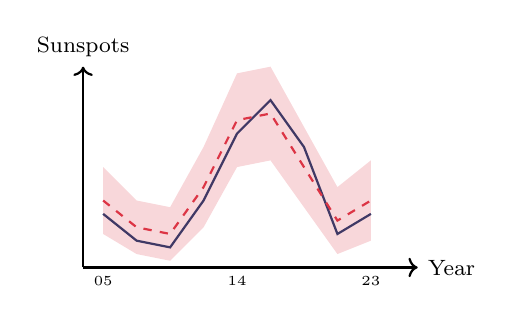
\begin{tikzpicture}[scale=0.85]
                \draw[thick, ->] (0,0) -- (5,0) node[right] {\footnotesize Year};
                \draw[thick, ->] (0,0) -- (0,3) node[above] {\footnotesize Sunspots};

                % Actual values (simplified)
                \draw[thick, MainBlue] (0.3,0.8) -- (0.8,0.4) -- (1.3,0.3) -- (1.8,1.0) -- (2.3,2.0) -- (2.8,2.5) -- (3.3,1.8) -- (3.8,0.5) -- (4.3,0.8);

                % Forecast
                \draw[thick, IDAred, dashed] (0.3,1.0) -- (0.8,0.6) -- (1.3,0.5) -- (1.8,1.2) -- (2.3,2.2) -- (2.8,2.3) -- (3.3,1.5) -- (3.8,0.7) -- (4.3,1.0);

                % Confidence band
                \fill[IDAred, opacity=0.2] (0.3,0.5) -- (0.8,0.2) -- (1.3,0.1) -- (1.8,0.6) -- (2.3,1.5) -- (2.8,1.6) -- (3.3,0.9) -- (3.8,0.2) -- (4.3,0.4) -- (4.3,1.6) -- (3.8,1.2) -- (3.3,2.1) -- (2.8,3.0) -- (2.3,2.9) -- (1.8,1.8) -- (1.3,0.9) -- (0.8,1.0) -- (0.3,1.5) -- cycle;

                % Labels
                \node[font=\tiny] at (0.3,-0.2) {05};
                \node[font=\tiny] at (2.3,-0.2) {14};
                \node[font=\tiny] at (4.3,-0.2) {23};
            \end{tikzpicture}

            \vspace{0.2em}
            {\footnotesize \textcolor{MainBlue}{---} Actual \quad \textcolor{IDAred}{- -} Forecast \quad \textcolor{IDAred!30}{$\blacksquare$} 95\% CI}
        \end{column}
    \end{columns}
\end{frame}

\begin{frame}{Sunspots: Summary}
    \begin{columns}[T]
        \begin{column}{0.48\textwidth}
            \textbf{Methodology:}
            \begin{enumerate}
                \item Split: 70/15/15 (years)
                \item Use Fourier terms for 11-year cycle
                \item Select K on validation (K=2 best)
                \item Final evaluation on test
            \end{enumerate}

            \vspace{0.5em}
            \textbf{Key Finding:}

            Fourier terms efficiently capture long seasonal patterns without losing data to differencing.
        \end{column}
        \begin{column}{0.48\textwidth}
            \textbf{Results:}
            \begin{table}[h]
                \footnotesize
                \begin{tabular}{ll}
                    \toprule
                    Best Model & ARIMA(2,0,1)+Fourier(2) \\
                    Validation RMSE & 24.2 \\
                    Test RMSE & 26.8 \\
                    Key insight & K=2 optimal \\
                    \bottomrule
                \end{tabular}
            \end{table}

            \vspace{0.5em}
            \begin{alertblock}{Lesson}
                For long seasonal periods:
                \begin{itemize}
                    \item Fourier terms > SARIMA
                    \item Select K via cross-validation
                \end{itemize}
            \end{alertblock}
        \end{column}
    \end{columns}
\end{frame}

%=============================================================================
% SECTION 4: CASE STUDY 3 - UNEMPLOYMENT
%=============================================================================
\section{Case Study 3: US Unemployment Forecasting}

\begin{frame}{Unemployment: Data and Challenge}
    \begin{columns}[T]
        \begin{column}{0.55\textwidth}
            \textbf{Data:} US Unemployment Rate (2010--2023)
            \begin{itemize}
                \item Source: FRED (UNRATE)
                \item 168 monthly observations
                \item Major structural break: COVID-19
            \end{itemize}

            \vspace{0.5em}
            \textbf{The Challenge:}
            \begin{itemize}
                \item April 2020: 3.5\% $\rightarrow$ 14.7\% (+10.3 pp)
                \item Largest single-month increase ever
                \item Traditional ARIMA struggles
            \end{itemize}

            \vspace{0.5em}
            \textbf{Solution:} Prophet with changepoint detection
        \end{column}
        \begin{column}{0.43\textwidth}
            \textbf{Data Split:}
            \begin{table}[h]
                \footnotesize
                \begin{tabular}{lcc}
                    \toprule
                    Set & Months & Period \\
                    \midrule
                    Training & 118 & 2010--2019 \\
                    Validation & 25 & 2020--2021 \\
                    Test & 25 & 2022--2023 \\
                    \bottomrule
                \end{tabular}
            \end{table}

            \vspace{0.3em}
            \begin{alertblock}{Note}
                Validation includes COVID shock --- tests model's adaptability
            \end{alertblock}
        \end{column}
    \end{columns}
\end{frame}

\begin{frame}{Prophet: Changepoint Detection}
    \textbf{Key Parameter:} \texttt{changepoint\_prior\_scale}

    \vspace{0.5em}
    \begin{columns}[T]
        \begin{column}{0.48\textwidth}
            \textbf{What it controls:}
            \begin{itemize}
                \item Flexibility of trend changes
                \item Low (0.01): Smooth, rigid trend
                \item High (0.5): Many changepoints allowed
            \end{itemize}

            \vspace{0.5em}
            \textbf{For COVID data:}
            \begin{itemize}
                \item Need flexibility for sudden jump
                \item But not too much (overfitting)
                \item \textcolor{Forest}{Select via validation!}
            \end{itemize}
        \end{column}
        \begin{column}{0.48\textwidth}
            \textbf{Prophet Model:}
            \[
                y(t) = g(t) + s(t) + h(t) + \epsilon_t
            \]

            Where:
            \begin{itemize}
                \item $g(t)$: Piecewise linear trend
                \item $s(t)$: Seasonality (Fourier)
                \item $h(t)$: Holiday effects
                \item Changepoints: Where $g(t)$ slope changes
            \end{itemize}
        \end{column}
    \end{columns}
\end{frame}

\begin{frame}{Unemployment: Model Selection on Validation Set}
    \textbf{Testing different \texttt{changepoint\_prior\_scale} values:}

    \vspace{0.5em}
    \begin{columns}[T]
        \begin{column}{0.55\textwidth}
            \begin{table}[h]
                \footnotesize
                \begin{tabular}{lccc}
                    \toprule
                    Scale & Changepoints & \textbf{Val RMSE} & Val MAE \\
                    \midrule
                    0.01 & 2 & 2.85 & 2.31 \\
                    0.05 & 4 & 1.92 & 1.54 \\
                    \textbf{0.10} & \textbf{5} & \textbf{1.24} & \textbf{0.98} \\
                    0.30 & 8 & 1.31 & 1.05 \\
                    0.50 & 12 & 1.48 & 1.19 \\
                    \bottomrule
                \end{tabular}
            \end{table}

            \vspace{0.3em}
            \textcolor{Forest}{$\Rightarrow$ Best: scale = 0.10}

            \vspace{0.3em}
            Detected changepoints:
            \begin{itemize}
                \item March 2020 (COVID start)
                \item April 2020 (peak)
                \item June 2020 (recovery start)
            \end{itemize}
        \end{column}
        \begin{column}{0.43\textwidth}
            \textbf{Why 0.10 wins:}
            \begin{itemize}
                \item Flexible enough for COVID
                \item Not overfitting to noise
                \item Balances bias/variance
            \end{itemize}

            \vspace{0.5em}
            \begin{exampleblock}{Key Insight}
                scale = 0.50 detected 12 changepoints --- too many!

                Model was chasing short-term noise.
            \end{exampleblock}
        \end{column}
    \end{columns}
\end{frame}

\begin{frame}{Unemployment: Final Test Set Evaluation}
    \textbf{Refit Prophet (scale=0.10) on Training+Validation, forecast Test (2022--2023)}

    \vspace{0.5em}
    \begin{columns}[T]
        \begin{column}{0.48\textwidth}
            \textbf{Test Set Results:}
            \begin{table}[h]
                \footnotesize
                \begin{tabular}{lc}
                    \toprule
                    Metric & Value \\
                    \midrule
                    Test RMSE & 0.42 \\
                    Test MAE & 0.35 \\
                    Test MAPE & 9.8\% \\
                    \bottomrule
                \end{tabular}
            \end{table}

            \vspace{0.5em}
            \textbf{Comparison with ARIMA:}
            \begin{table}[h]
                \footnotesize
                \begin{tabular}{lcc}
                    \toprule
                    Model & Test RMSE \\
                    \midrule
                    ARIMA(2,1,2) & 0.89 \\
                    \textbf{Prophet} & \textbf{0.42} \\
                    \bottomrule
                \end{tabular}
            \end{table}
        \end{column}
        \begin{column}{0.48\textwidth}
            \textbf{Forecast Visualization (2022--2023):}

            \vspace{0.3em}
            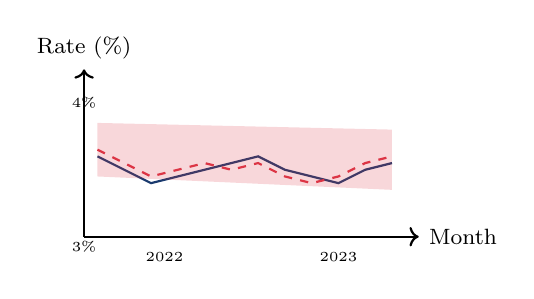
\begin{tikzpicture}[scale=0.85]
                \draw[thick, ->] (0,0) -- (5,0) node[right] {\footnotesize Month};
                \draw[thick, ->] (0,0) -- (0,2.5) node[above] {\footnotesize Rate (\%)};

                % Axis labels
                \node[font=\tiny] at (0,-0.15) {3\%};
                \node[font=\tiny] at (0,2) {4\%};

                % Actual values
                \draw[thick, MainBlue] (0.2,1.2) -- (0.6,1.0) -- (1,0.8) -- (1.4,0.9) -- (1.8,1.0) -- (2.2,1.1) -- (2.6,1.2) -- (3,1.0) -- (3.4,0.9) -- (3.8,0.8) -- (4.2,1.0) -- (4.6,1.1);

                % Forecast
                \draw[thick, IDAred, dashed] (0.2,1.3) -- (0.6,1.1) -- (1,0.9) -- (1.4,1.0) -- (1.8,1.1) -- (2.2,1.0) -- (2.6,1.1) -- (3,0.9) -- (3.4,0.8) -- (3.8,0.9) -- (4.2,1.1) -- (4.6,1.2);

                % CI band
                \fill[IDAred, opacity=0.2] (0.2,0.9) -- (4.6,0.7) -- (4.6,1.6) -- (0.2,1.7) -- cycle;

                % Year labels
                \node[font=\tiny] at (1.2,-0.3) {2022};
                \node[font=\tiny] at (3.8,-0.3) {2023};
            \end{tikzpicture}

            \vspace{0.2em}
            {\footnotesize \textcolor{MainBlue}{---} Actual \quad \textcolor{IDAred}{- -} Prophet}
        \end{column}
    \end{columns}
\end{frame}

\begin{frame}{Unemployment: Summary}
    \begin{columns}[T]
        \begin{column}{0.48\textwidth}
            \textbf{Methodology:}
            \begin{enumerate}
                \item Split: 70/15/15 (months)
                \item Tune \texttt{changepoint\_prior\_scale}
                \item Select optimal scale on validation
                \item Final evaluation on test
            \end{enumerate}

            \vspace{0.5em}
            \textbf{Key Finding:}

            Prophet handles structural breaks better than ARIMA through automatic changepoint detection.
        \end{column}
        \begin{column}{0.48\textwidth}
            \textbf{Results:}
            \begin{table}[h]
                \footnotesize
                \begin{tabular}{ll}
                    \toprule
                    Best Model & Prophet (scale=0.10) \\
                    Validation RMSE & 1.24 \\
                    Test RMSE & 0.42 \\
                    vs ARIMA & 53\% better \\
                    \bottomrule
                \end{tabular}
            \end{table}

            \vspace{0.5em}
            \begin{alertblock}{Lesson}
                For data with structural breaks:
                \begin{itemize}
                    \item Prophet > traditional ARIMA
                    \item Tune changepoint flexibility
                \end{itemize}
            \end{alertblock}
        \end{column}
    \end{columns}
\end{frame}

%=============================================================================
% SECTION 5: CASE STUDY 4 - VAR MULTIVARIATE
%=============================================================================
\section{Case Study 4: Multivariate VAR Forecasting}

\begin{frame}{VAR: Data and Objective}
    \begin{columns}[T]
        \begin{column}{0.55\textwidth}
            \textbf{Data:} US Economic Indicators (2001--2023)
            \begin{itemize}
                \item Source: FRED
                \item 92 quarterly observations
                \item 4 variables (GDP, Unemp, Inflation, Fed Rate)
            \end{itemize}

            \vspace{0.5em}
            \textbf{Objective:} Joint forecasting + relationship analysis

            \vspace{0.5em}
            \textbf{Why VAR?}
            \begin{itemize}
                \item Variables influence each other
                \item Feedback loops (GDP $\leftrightarrow$ Unemployment)
                \item Policy transmission (Fed $\rightarrow$ Economy)
            \end{itemize}
        \end{column}
        \begin{column}{0.43\textwidth}
            \textbf{Data Split:}
            \begin{table}[h]
                \footnotesize
                \begin{tabular}{lcc}
                    \toprule
                    Set & Quarters & Period \\
                    \midrule
                    Training & 64 & 2001--2016 \\
                    Validation & 14 & 2017--2020 \\
                    Test & 14 & 2021--2023 \\
                    \bottomrule
                \end{tabular}
            \end{table}

            \vspace{0.3em}
            \textbf{Variables:}
            \begin{itemize}
                \item GDP Growth (YoY \%)
                \item Unemployment (\%)
                \item Inflation (CPI YoY \%)
                \item Fed Funds Rate (\%)
            \end{itemize}
        \end{column}
    \end{columns}
\end{frame}

\begin{frame}{VAR: Lag Order Selection on Validation}
    \textbf{VAR(p) Model:}
    $\mathbf{y}_t = \mathbf{c} + \mathbf{A}_1 \mathbf{y}_{t-1} + \cdots + \mathbf{A}_p \mathbf{y}_{t-p} + \boldsymbol{\varepsilon}_t$

    \vspace{0.5em}
    \begin{columns}[T]
        \begin{column}{0.55\textwidth}
            \textbf{Selecting lag order p:}
            \begin{table}[h]
                \footnotesize
                \begin{tabular}{lcccc}
                    \toprule
                    Lag & AIC & BIC & \textbf{Val RMSE} \\
                    \midrule
                    1 & 12.4 & 13.1 & 1.85 \\
                    \textbf{2} & \textbf{11.8} & \textbf{13.0} & \textbf{1.42} \\
                    3 & 11.6 & 13.4 & 1.51 \\
                    4 & 11.5 & 13.8 & 1.68 \\
                    \bottomrule
                \end{tabular}
            \end{table}

            \vspace{0.3em}
            \textcolor{Forest}{$\Rightarrow$ Best: VAR(2)}

            \vspace{0.3em}
            Higher lags: lower AIC but higher validation error (overfitting)
        \end{column}
        \begin{column}{0.43\textwidth}
            \textbf{VAR(2) Parameters:}
            \begin{itemize}
                \item 4 variables $\times$ 2 lags = 8 coeff per equation
                \item + 4 intercepts
                \item Total: 36 parameters
            \end{itemize}

            \vspace{0.5em}
            \begin{alertblock}{BIC vs AIC}
                BIC selects p=2 (simpler)

                AIC selects p=3 (complex)

                Validation confirms BIC!
            \end{alertblock}
        \end{column}
    \end{columns}
\end{frame}

\begin{frame}{VAR: Granger Causality Results}
    \textbf{Testing predictive relationships (on Training data):}

    \vspace{0.5em}
    \begin{columns}[T]
        \begin{column}{0.55\textwidth}
            \begin{table}[h]
                \footnotesize
                \begin{tabular}{lccc}
                    \toprule
                    Cause $\rightarrow$ Effect & F-stat & p-value & Sig. \\
                    \midrule
                    GDP $\rightarrow$ Unemployment & 4.82 & 0.012 & ** \\
                    Unemployment $\rightarrow$ GDP & 1.45 & 0.243 & \\
                    Inflation $\rightarrow$ Fed Rate & 6.21 & 0.004 & ** \\
                    Fed Rate $\rightarrow$ Inflation & 2.88 & 0.065 & * \\
                    GDP $\rightarrow$ Inflation & 3.12 & 0.052 & * \\
                    Fed $\rightarrow$ Unemployment & 2.15 & 0.127 & \\
                    \bottomrule
                \end{tabular}
            \end{table}

            {\footnotesize ** p<0.05, * p<0.10}
        \end{column}
        \begin{column}{0.43\textwidth}
            \textbf{Interpretation:}
            \begin{itemize}
                \item GDP leads unemployment (Okun's Law confirmed)
                \item Inflation leads Fed policy (Taylor Rule)
                \item Bidirectional: Fed $\leftrightarrow$ Inflation
            \end{itemize}

            \vspace{0.3em}
            \begin{exampleblock}{Caution}
                Granger causality = predictive, not true causality!
            \end{exampleblock}
        \end{column}
    \end{columns}
\end{frame}

\begin{frame}{VAR: Final Test Set Evaluation}
    \textbf{Refit VAR(2) on Training+Validation, forecast Test (2021--2023)}

    \vspace{0.5em}
    \begin{columns}[T]
        \begin{column}{0.55\textwidth}
            \textbf{Test Set Results (by variable):}
            \begin{table}[h]
                \footnotesize
                \begin{tabular}{lccc}
                    \toprule
                    Variable & RMSE & MAE & vs AR(2) \\
                    \midrule
                    GDP Growth & 1.82 & 1.45 & -18\% \\
                    Unemployment & 0.58 & 0.44 & -25\% \\
                    Inflation & 1.24 & 0.98 & -12\% \\
                    Fed Rate & 0.89 & 0.72 & -31\% \\
                    \midrule
                    \textbf{Average} & \textbf{1.13} & \textbf{0.90} & \textbf{-22\%} \\
                    \bottomrule
                \end{tabular}
            \end{table}

            \vspace{0.3em}
            VAR(2) beats univariate AR(2) by 22\% on average!
        \end{column}
        \begin{column}{0.43\textwidth}
            \textbf{Why VAR wins:}
            \begin{itemize}
                \item Uses cross-variable information
                \item GDP helps predict unemployment
                \item Inflation helps predict Fed
            \end{itemize}

            \vspace{0.5em}
            \begin{exampleblock}{Best Improvement}
                Fed Rate: -31\% RMSE

                Why? Inflation is a strong leading indicator for Fed policy.
            \end{exampleblock}
        \end{column}
    \end{columns}
\end{frame}

\begin{frame}{VAR: Impulse Response Analysis}
    \textbf{How does a 1\% GDP shock affect other variables?}

    \vspace{0.3em}
    \begin{center}
        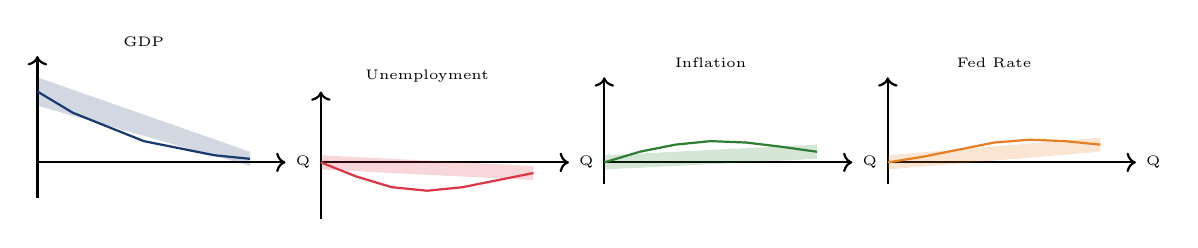
\begin{tikzpicture}[scale=0.9]
            % GDP response
            \begin{scope}[shift={(0,0)}]
                \draw[thick, ->] (0,0) -- (3.5,0) node[right] {\tiny Q};
                \draw[thick, ->] (0,-0.5) -- (0,1.5);
                \node[font=\tiny, above] at (1.5,1.5) {GDP};
                \draw[thick, MainBlue] (0,1) -- (0.5,0.7) -- (1,0.5) -- (1.5,0.3) -- (2,0.2) -- (2.5,0.1) -- (3,0.05);
                \fill[MainBlue, opacity=0.2] (0,1.2) -- (3,0.15) -- (3,-0.05) -- (0,0.8) -- cycle;
            \end{scope}

            % Unemployment response
            \begin{scope}[shift={(4,0)}]
                \draw[thick, ->] (0,0) -- (3.5,0) node[right] {\tiny Q};
                \draw[thick, ->] (0,-0.8) -- (0,1);
                \node[font=\tiny, above] at (1.5,1) {Unemployment};
                \draw[thick, IDAred] (0,0) -- (0.5,-0.2) -- (1,-0.35) -- (1.5,-0.4) -- (2,-0.35) -- (2.5,-0.25) -- (3,-0.15);
                \fill[IDAred, opacity=0.2] (0,0.1) -- (3,-0.05) -- (3,-0.25) -- (0,-0.1) -- cycle;
            \end{scope}

            % Inflation response
            \begin{scope}[shift={(8,0)}]
                \draw[thick, ->] (0,0) -- (3.5,0) node[right] {\tiny Q};
                \draw[thick, ->] (0,-0.3) -- (0,1.2);
                \node[font=\tiny, above] at (1.5,1.2) {Inflation};
                \draw[thick, Forest] (0,0) -- (0.5,0.15) -- (1,0.25) -- (1.5,0.3) -- (2,0.28) -- (2.5,0.22) -- (3,0.15);
                \fill[Forest, opacity=0.2] (0,0.1) -- (3,0.25) -- (3,0.05) -- (0,-0.1) -- cycle;
            \end{scope}

            % Fed response
            \begin{scope}[shift={(12,0)}]
                \draw[thick, ->] (0,0) -- (3.5,0) node[right] {\tiny Q};
                \draw[thick, ->] (0,-0.3) -- (0,1.2);
                \node[font=\tiny, above] at (1.5,1.2) {Fed Rate};
                \draw[thick, Orange] (0,0) -- (0.5,0.08) -- (1,0.18) -- (1.5,0.28) -- (2,0.32) -- (2.5,0.3) -- (3,0.25);
                \fill[Orange, opacity=0.2] (0,0.1) -- (3,0.35) -- (3,0.15) -- (0,-0.1) -- cycle;
            \end{scope}
        \end{tikzpicture}
    \end{center}

    \vspace{0.3em}
    \textbf{Interpretation (from IRF):}
    \begin{itemize}
        \item GDP shock $\Rightarrow$ Unemployment falls for 4-6 quarters (Okun's Law)
        \item GDP shock $\Rightarrow$ Inflation rises, peaks at Q3-Q4 (demand-pull)
        \item GDP shock $\Rightarrow$ Fed Rate rises with lag (policy response)
    \end{itemize}
\end{frame}

\begin{frame}{VAR: Summary}
    \begin{columns}[T]
        \begin{column}{0.48\textwidth}
            \textbf{Methodology:}
            \begin{enumerate}
                \item Split: 70/15/15 (quarters)
                \item Select lag order on validation (p=2)
                \item Test Granger causality
                \item Analyze IRF
                \item Final forecast on test
            \end{enumerate}

            \vspace{0.5em}
            \textbf{Key Finding:}

            VAR captures economic interdependencies that univariate models miss.
        \end{column}
        \begin{column}{0.48\textwidth}
            \textbf{Results:}
            \begin{table}[h]
                \footnotesize
                \begin{tabular}{ll}
                    \toprule
                    Best Model & VAR(2) \\
                    Validation RMSE & 1.42 \\
                    Test RMSE & 1.13 \\
                    vs Univariate & 22\% better \\
                    \bottomrule
                \end{tabular}
            \end{table}

            \vspace{0.5em}
            \begin{exampleblock}{Applications}
                \begin{itemize}
                    \item Macroeconomic forecasting
                    \item Policy impact analysis
                    \item Portfolio risk (multi-asset)
                \end{itemize}
            \end{exampleblock}
        \end{column}
    \end{columns}
\end{frame}

%=============================================================================
% SECTION 6: MODEL SELECTION GUIDE
%=============================================================================
\section{Model Selection: A Practical Guide}

\begin{frame}{Decision Framework}
    \begin{center}
        \includegraphics[width=0.90\textwidth, height=0.70\textheight, keepaspectratio]{ch10_model_selection_flowchart.pdf}
    \end{center}
\end{frame}

\begin{frame}{Model Selection Summary}
    \begin{table}[h]
        \footnotesize
        \centering
        \begin{tabular}{p{2.5cm}p{3.5cm}p{3.5cm}p{3cm}}
            \toprule
            \textbf{Data Type} & \textbf{Characteristics} & \textbf{Recommended Model} & \textbf{Alternatives} \\
            \midrule
            Financial returns & No trend, volatility clustering & ARIMA-GARCH & EGARCH, GJR \\
            \addlinespace
            Single seasonality & Trend + one seasonal period & SARIMA & ETS, Prophet \\
            \addlinespace
            Long cycles & Sunspots, business cycles & AR + Fourier, TBATS & Spectral methods \\
            \addlinespace
            Structural breaks & COVID, regime changes & Prophet & Intervention ARIMA \\
            \addlinespace
            Multiple series & Interdependencies & VAR, VECM & Factor models \\
            \bottomrule
        \end{tabular}
    \end{table}
\end{frame}

\begin{frame}{Forecast Evaluation Metrics}
    \begin{columns}[T]
        \begin{column}{0.48\textwidth}
            \textbf{Point Forecast Metrics:}

            \vspace{0.3em}
            \textbf{RMSE} (Root Mean Square Error):
            \[
                \sqrt{\frac{1}{n}\sum_{i=1}^{n}(y_i - \hat{y}_i)^2}
            \]

            \textbf{MAE} (Mean Absolute Error):
            \[
                \frac{1}{n}\sum_{i=1}^{n}|y_i - \hat{y}_i|
            \]

            \textbf{MAPE} (Mean Absolute \% Error):
            \[
                \frac{100}{n}\sum_{i=1}^{n}\left|\frac{y_i - \hat{y}_i}{y_i}\right|
            \]
        \end{column}
        \begin{column}{0.48\textwidth}
            \textbf{When to Use Each:}
            \begin{itemize}
                \item \textbf{RMSE}: Penalizes large errors more
                \item \textbf{MAE}: Robust to outliers
                \item \textbf{MAPE}: Scale-independent
            \end{itemize}

            \vspace{0.5em}
            \begin{alertblock}{Cross-Validation}
                Always use time series CV:
                \begin{itemize}
                    \item Rolling window
                    \item Expanding window
                    \item Never shuffle!
                \end{itemize}
            \end{alertblock}
        \end{column}
    \end{columns}
\end{frame}

%=============================================================================
% SECTION 6: SUMMARY
%=============================================================================
\section{Summary and Key Takeaways}

\begin{frame}{Course Summary: Complete Toolkit}
    \begin{columns}[T]
        \begin{column}{0.48\textwidth}
            \textbf{Understanding the Data}
            \begin{itemize}
                \item Visualization first!
                \item Test for stationarity (ADF, KPSS)
                \item Identify seasonality patterns
                \item Check for structural breaks
            \end{itemize}

            \vspace{0.5em}
            \textbf{Classical Models}
            \begin{itemize}
                \item ARIMA: Non-seasonal data
                \item SARIMA: Single seasonality
                \item GARCH: Volatility modeling
            \end{itemize}
        \end{column}
        \begin{column}{0.48\textwidth}
            \textbf{Modern Approaches}
            \begin{itemize}
                \item Prophet: Interpretable, handles breaks
                \item TBATS: Multiple/long seasonalities
                \item VAR/VECM: Multiple time series
            \end{itemize}

            \vspace{0.5em}
            \textbf{Best Practices}
            \begin{itemize}
                \item Always check diagnostics
                \item Use cross-validation
                \item Compare multiple models
                \item Domain knowledge matters!
            \end{itemize}
        \end{column}
    \end{columns}
\end{frame}

\begin{frame}{Final Recommendations}
    \begin{enumerate}
        \item \textbf{Start Simple}: Begin with visualization and basic statistics
        \item \textbf{Test Assumptions}: Stationarity, normality, independence
        \item \textbf{Iterate}: Model $\rightarrow$ Diagnose $\rightarrow$ Improve
        \item \textbf{Compare}: Never rely on a single model
        \item \textbf{Validate}: Out-of-sample testing is essential
        \item \textbf{Communicate}: Clear visualizations and interpretations
    \end{enumerate}

    \vspace{0.5em}
    \begin{exampleblock}{Remember}
        ``All models are wrong, but some are useful.'' --- George Box

        \vspace{0.3em}
        The goal is not perfect prediction, but useful insights and reasonable forecasts.
    \end{exampleblock}
\end{frame}

\begin{frame}{Questions?}
    \begin{center}
        \Large\textcolor{MainBlue}{Questions?}

        \vspace{1cm}

        \normalsize
        \textbf{Next Steps:}
        \begin{itemize}
            \item Practice with the Jupyter notebook
            \item Apply these methods to your own data
            \item Compare different models on the same dataset
        \end{itemize}

        \vspace{0.5cm}

        Course Materials: \texttt{github.com/danpele/Time-Series-Analysis}
    \end{center}
\end{frame}

\end{document}
